\chapter{Main Body}
\label{cha:Main Body}


\section{''Pflichtenheft''}
\label{sec:Pflichtenheft}

\subsubsection{Cost}
I've already bought two \acs{devboard}s one of them stays at \acs{tbz} and the other is at home. One of these boards was paid by Mr. Malacarne. Further expenses from the \acs{pcb} will be paid by me and shouldn't exceed about 50 CHF, as the \acs{hw} isn't that complicated.

\subsubsection{Time}
The most time of the project I will work at home because it's a rather big project to execute in one semester. I will also have much time in the fall holidays to work on it. The project will approximately take 100h to complete. Also the more detailed timeplan is in chapter: [\ref{sec:GANTT Chart}]

\subsubsection{Tools}
To realize this project I will mainly use, the \acs{sw} STM32CubeIDE with \acs{hal} and Altium Designer. The documentation is written in LaTeX in VSCode. And I'm planning to order the \acs{pcb} on JLCPCB and I will populate and reflow the PCB at ETHZ, where I'm also allowed to use the measurement equipment for the HW tests.

\subsubsection{Technical Details}
\begin{table}[H]
    \centering
    \label{tab:Technical Details}
\begin{tabular}{||c || c | c | c | c  || c ||} 
 \hline
 value &  min. & typ. & max. & unit & description \\ [0.5ex] 
 \hline\hline
  supply voltage & & 5 & & V & over USB \\ 
 \hline
 curent to measure & 0 & & 1 & A & \\ 
 \hline
 voltage to measure & 0 & & 10 & V & \\ 
 \hline
\end{tabular}
    \caption{Technical Details}
\end{table}

\newpage


\section{Extension PCB}
\label{sec:Extension PCB}



\subsection{STMod+}
Interface from DevBoard to Extension PCB. 

\begin{itemize}
    \item 5V Supply
    \item SPI 
    \item I\textsubscript{2}C
    \item ADC
    \item Interrupt
    \item PWM
    \item GPIOs
\end{itemize}

I will use the STMOD\#14 connection that was intended to use as PWM, as a second ADC input. To measure current and voltage at the same time to later show the power cosumption of the DUT.

\begin{figure}[H]
	\centering
	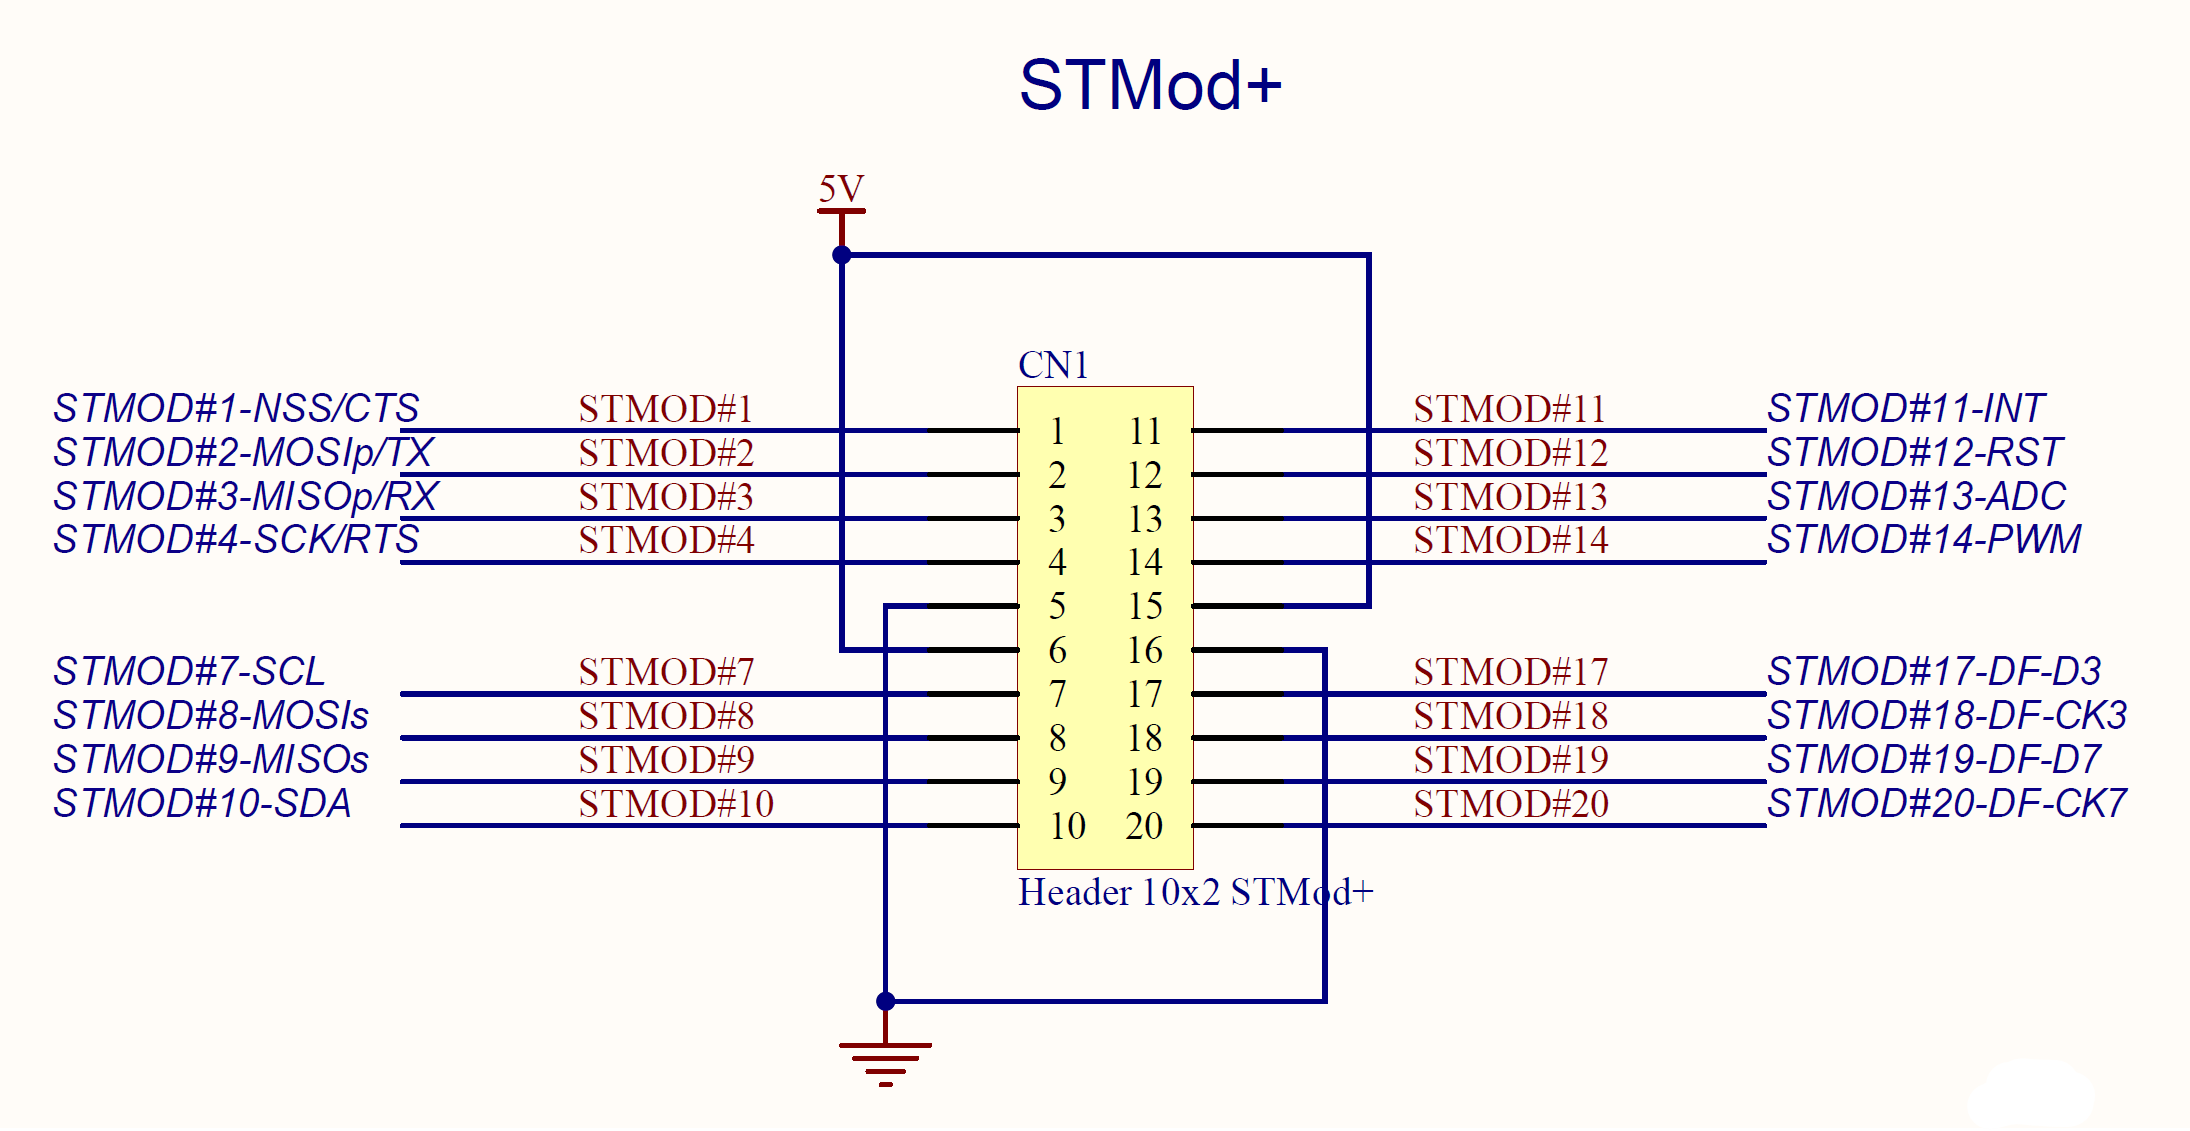
\includegraphics[width=13cm]{Resources/STMOD_Interface.png}
	\caption{STMod+ Interface}
	\label{fig:STMod+ Interface}
\end{figure}




\newpage

\subsection{Hardware concept}

After some thoughts I came up with the following HW concept.


\begin{figure}[H]
	\centering



    \tikzstyle{block} = [draw, fill=white, rectangle, 
    minimum height=3em, minimum width=6em]
    \tikzstyle{sum} = [draw, fill=white, circle, node distance=1cm]
    \tikzstyle{input} = [coordinate]
    \tikzstyle{output} = [coordinate]
    \tikzstyle{pinstyle} = [pin edge={to-,thin,black}]

    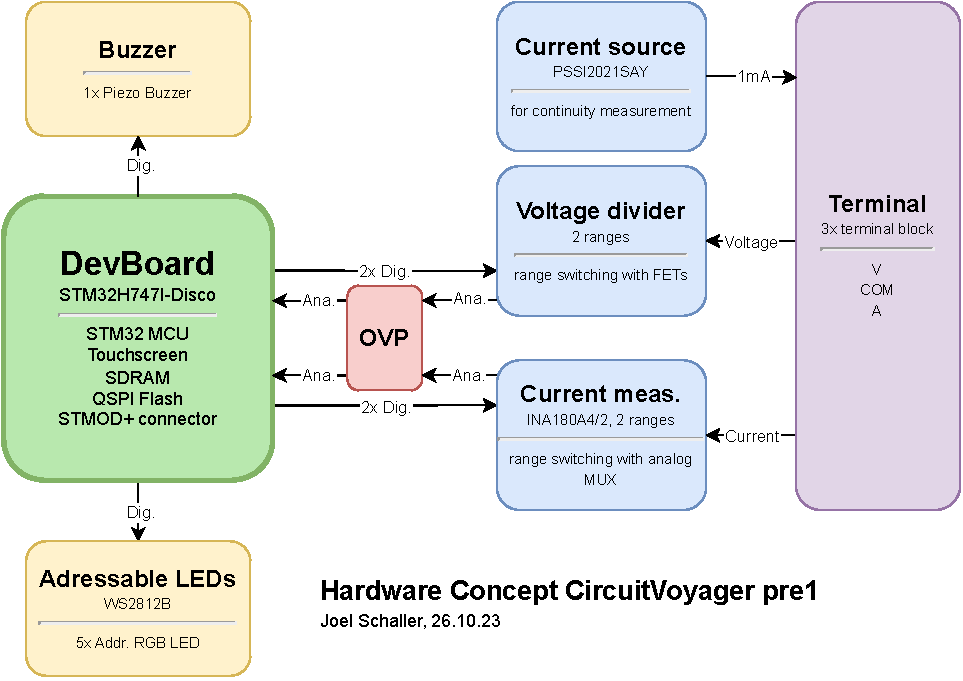
\includegraphics[width=15cm]{../../2_Project_Planning/HW_Concept/Hardware_Concept_CircuitVoyager_pre1.pdf}

    \vspace{0.2cm}

	\caption{Extension PCB HW concept}
	\label{fig:Extension PCB HW concept}
\end{figure}

\subsubsection{Voltage measurement}
To measure voltage, the DUT should be connected to the terminals V and COM. COM is connected internally to device GND. The V terminal is connected to the Voltage divider block. This block divides the input voltage down, so the ADC in the MCU doesn't overshoot. There are 2 ranges to measure voltage, which can be chosen by setting 2 digital output, that go from the MCU to the voltage divider. There's also an OVP, to protect the MCU from voltages higher than 3.3V. \cite{DMM_Video_ElectroNoobs}

\subsubsection{Current measurement}
To measure current, the DUT should be connected to the terminals A and COM. COM is connected internally to device GND. The A terminal is connected to current measurement block. This block measures the current, by letting the current flow through one of two shunt resistors. The DMM can choose which resistor and therefore range should be selected with the 2 digital Output that are connected from the MCU to the current measurement block. The voltage over the selected shunt is then amplified, by a current amplifier IC and then measured by the MCUs ADC. There's also an OVP, to protect the MCU from voltages higher than 3.3V. \cite{DMM_Video_ElectroNoobs}

\subsubsection{Continuity measurement}
To measure continuity, both the voltage divider and the current source is used. The continuity between the V and COM pins is measured. For this a constant current produced by the current source is flowing out of the V terminal. Simultaneously the voltage across those terminals is measured and the resistance / continuity can be evaluated. If continuity is detected, either the buzzer beeps or the LEDs blink. \cite{DMM_Video_ElectroNoobs}



\subsection{Schematic}
The schematic took me a bit longer than usual, because it's my first whole HW project in Altium before I used KiCAD and Altium is a lot more features and in my opinion is harder to learn. The schematic is in the Appendix \ref{sec:Extension PCB Schematics}.

\subsubsection{Buzzer Circuit}

\begin{figure}[H]
	\centering
	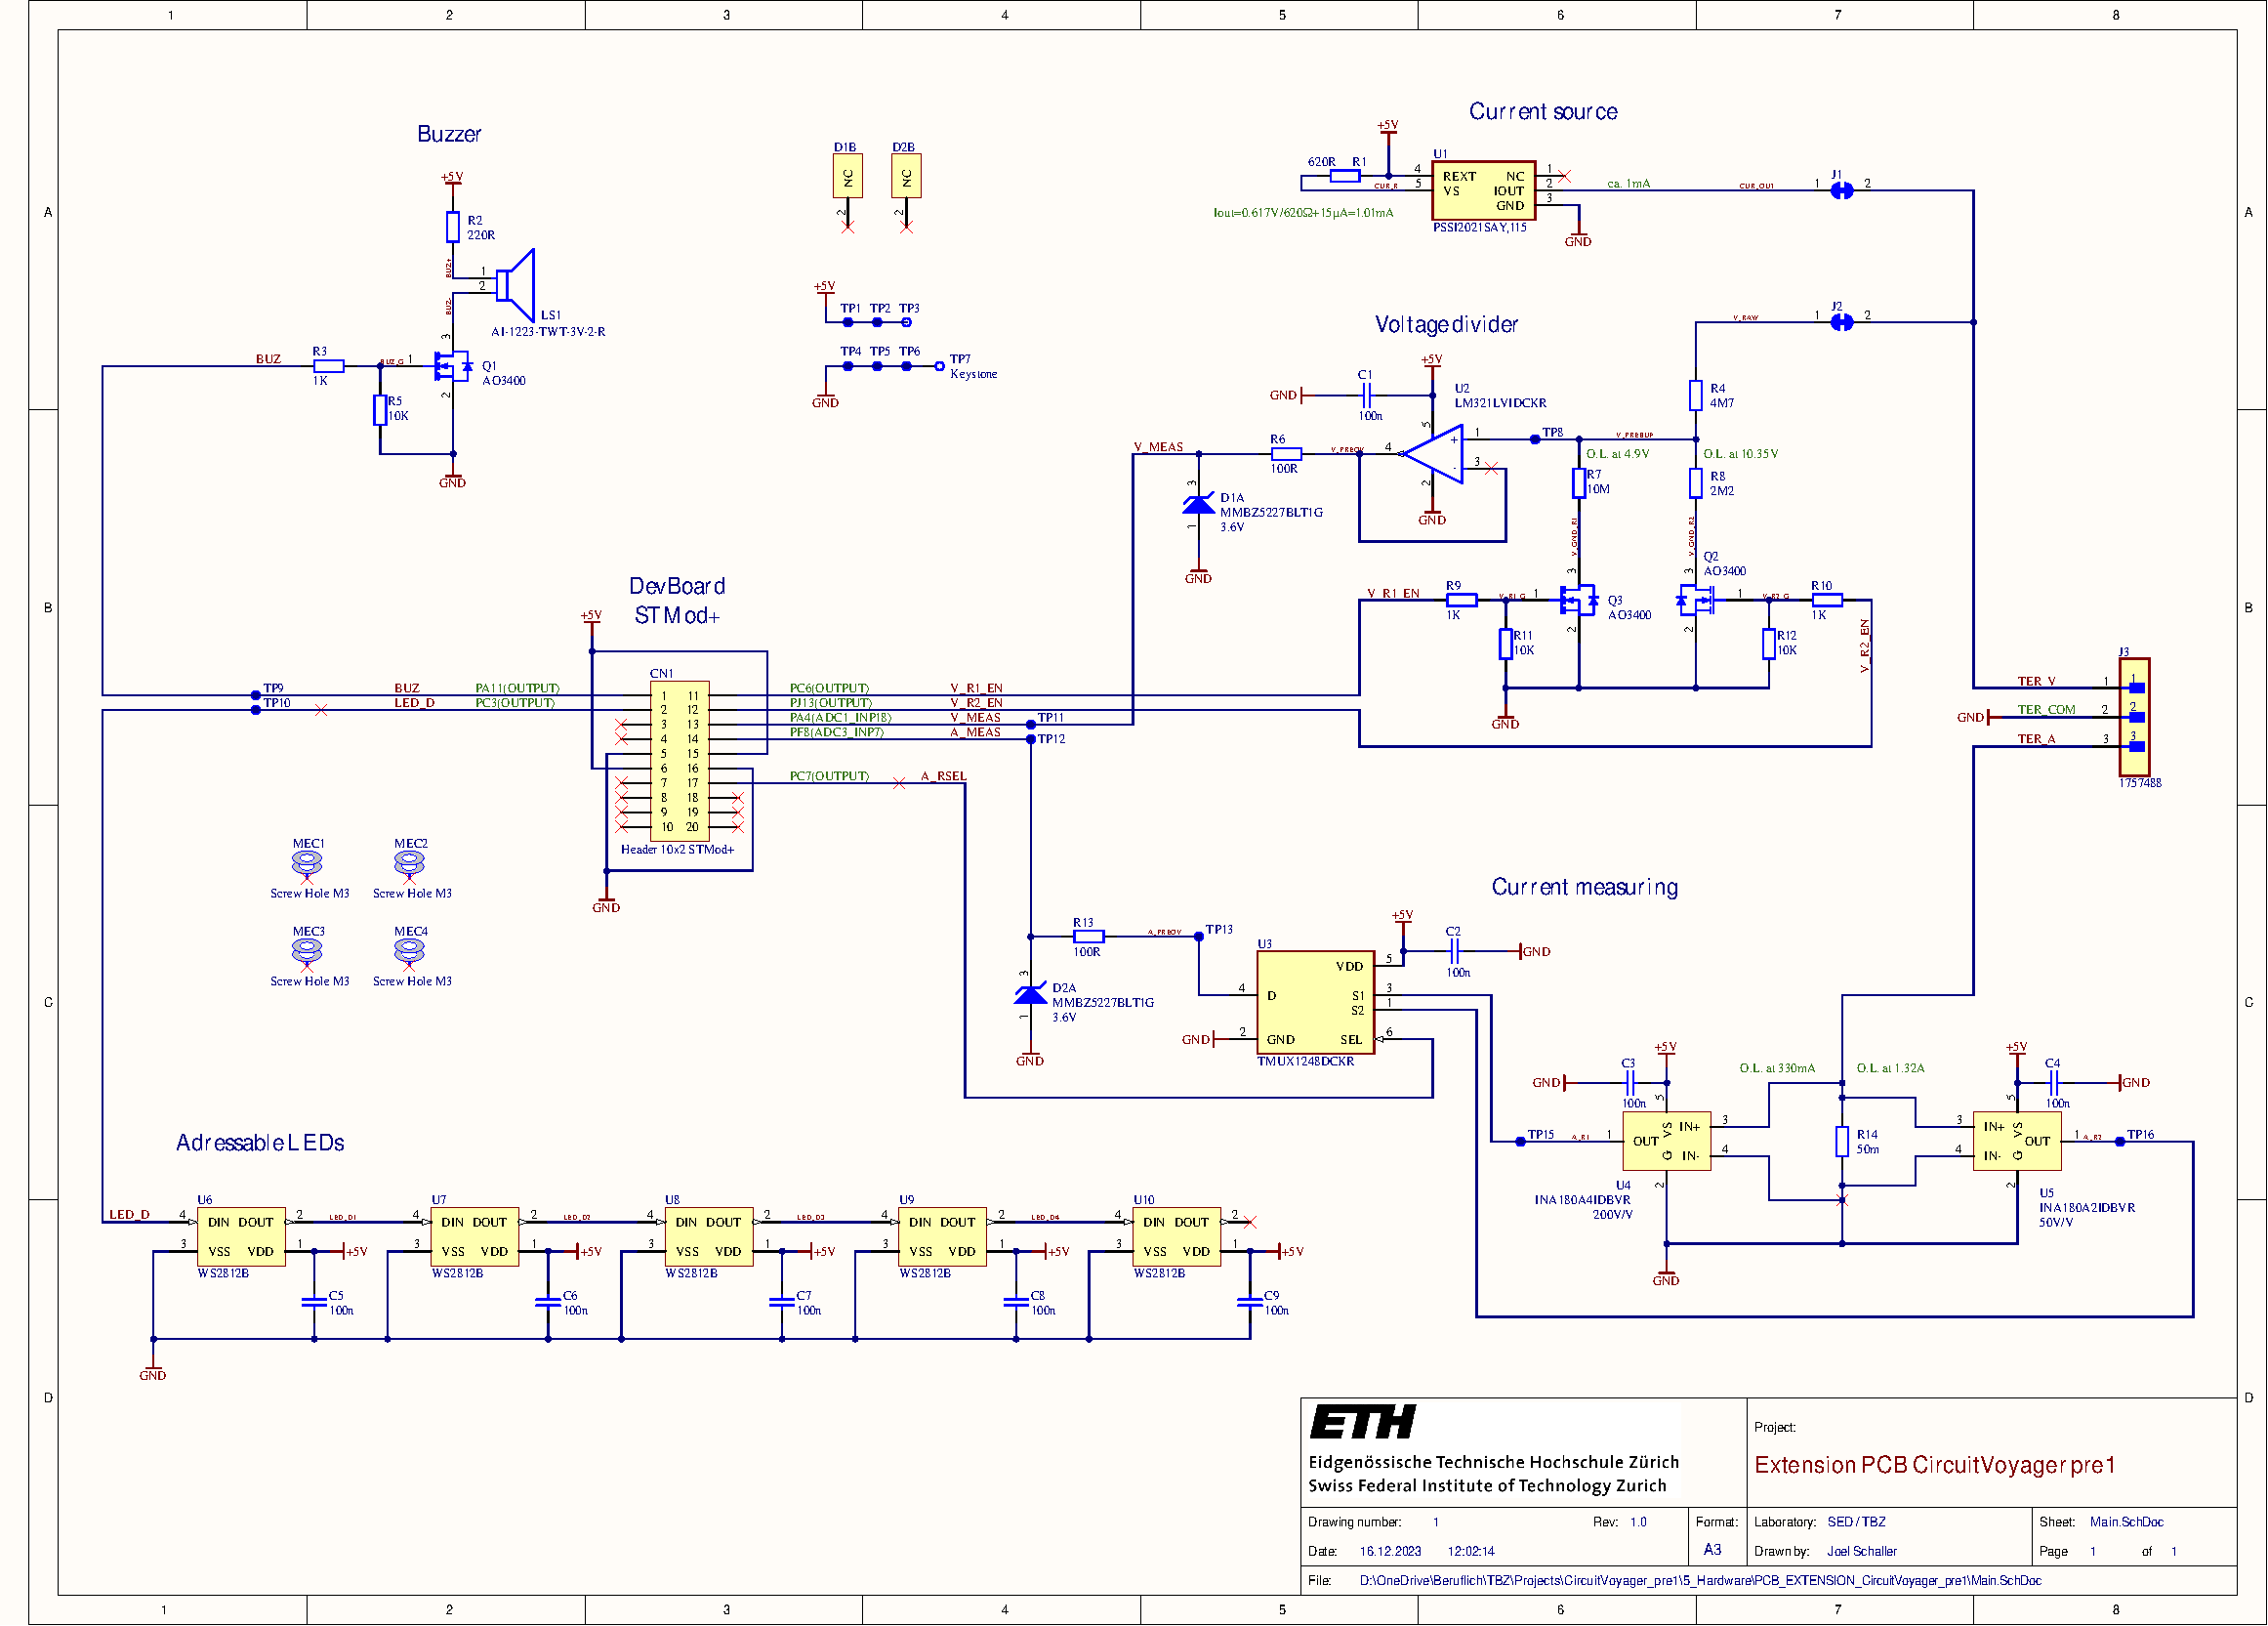
\includegraphics[width=8cm, trim={3.4cm 19cm 28.5cm 2cm}, clip]{../../../5_Hardware/PCB_EXTENSION_CircuitVoyager_pre1/Project Outputs for PCB_EXT_CV_PRE1/Schematic_PCB_EXTENSION_CircuitVoyager_pre1.pdf}
	\caption{Buzzer Circuit}
	\label{fig:Buzzer Circuit}
\end{figure}

This is an active buzzer. If the BUZ line is pulled high by the MCU, the MOSFET starts to conduct and the buzzer starts beeping. This circuit will be used to give an acoustic feedback to the user, if for example a continuity has been detected. 

The resistors R3 and R5 build a voltage divider with a ratio of 1/10. This has the advantage, that the gate capacitance of Q1 is charged with a limited current and if nothing's connected to the BUZ net the MOSFET turns the buzzer off and the whole machine isn't  in an indeterminate state.

The resistor R2 limit the current flowing through LS1. As LS1 is rated for 30mA at 3V.
\[R_2=\frac{U_{VCC}-U_{LS1}}{I_{LS1}}=\frac{5V-3V}{30mA}=66.\overline{6}\Omega\]

\[P_{R2}=I^2 \cdot R=(30mA)^2 \cdot 66. \overline{6} \Omega =60mW\]
Finally, I've chosen a 220\(\Omega\) resistor for R2. With this value the sound should be enough loud, that the user hears it. And the power loss of the resistor will be smaller. That means it should be perfectly fine to use a 0402 resistor that is rated for 62.5mW.


\subsubsection{Adressable LEDs Circuit}

\begin{figure}[H]
	\centering
	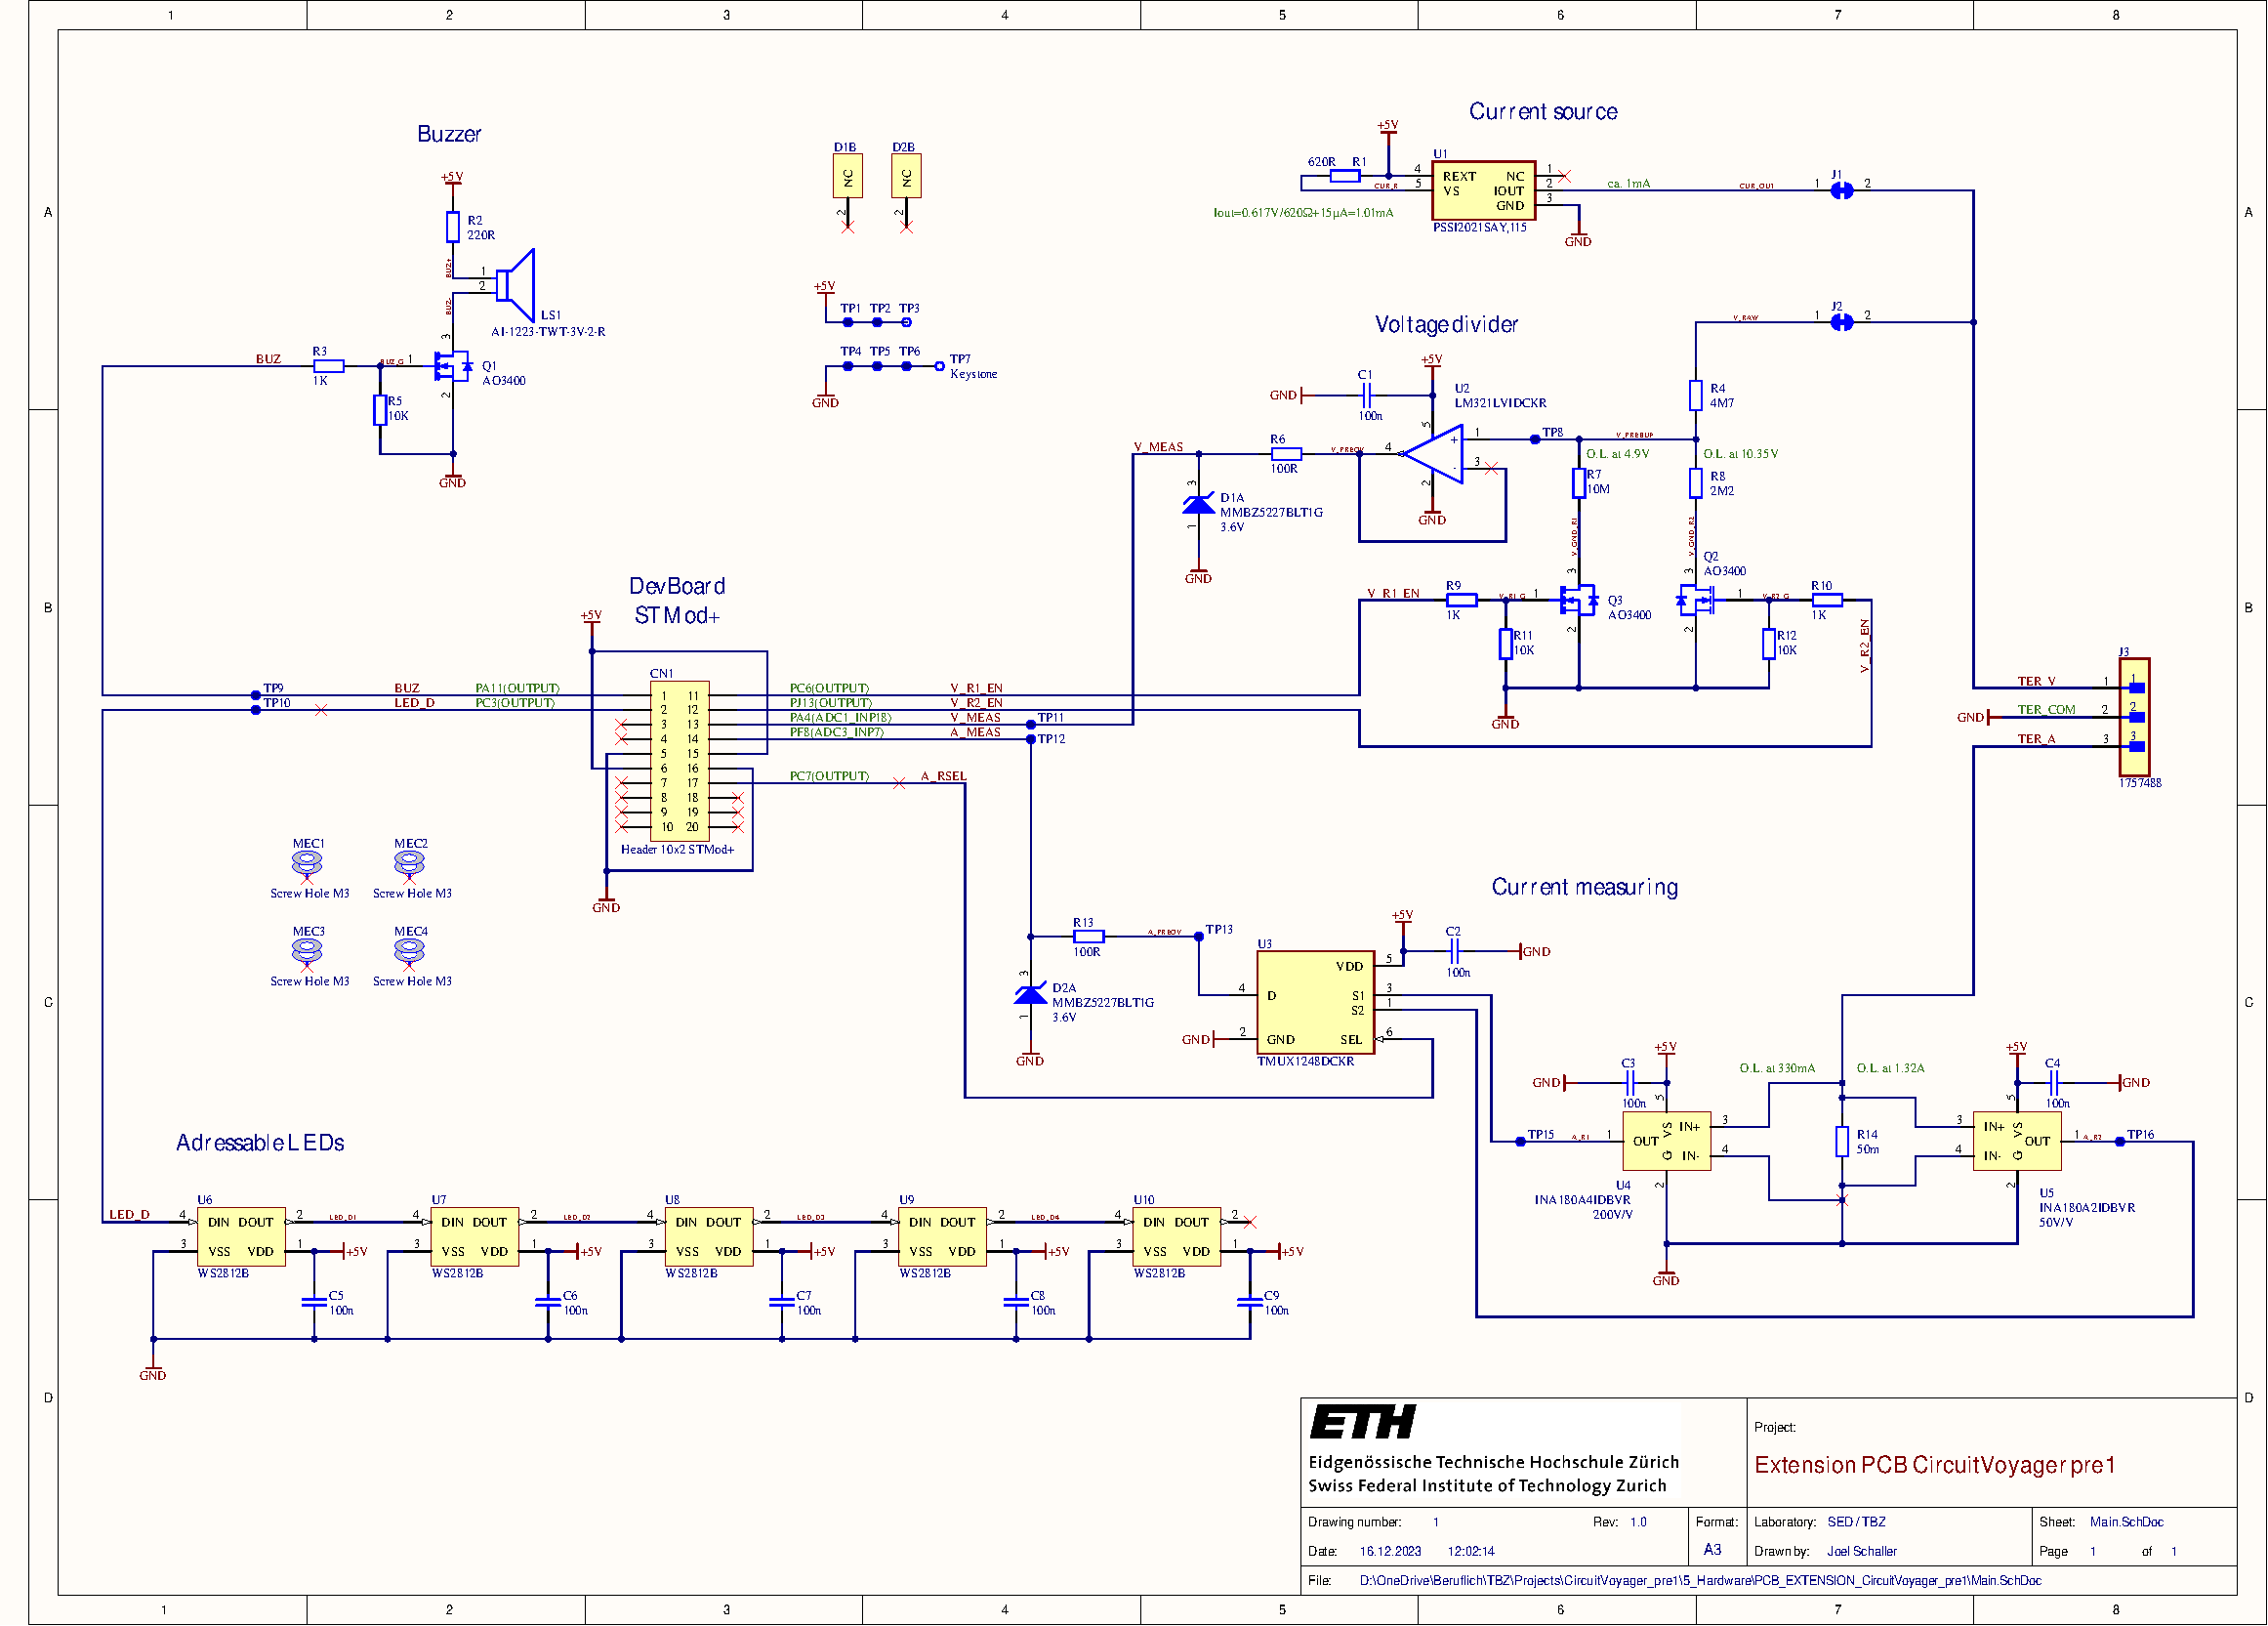
\includegraphics[width=15cm, trim={1.3cm 4cm 16.3cm 20cm}, clip]{../../../5_Hardware/PCB_EXTENSION_CircuitVoyager_pre1/Project Outputs for PCB_EXT_CV_PRE1/Schematic_PCB_EXTENSION_CircuitVoyager_pre1.pdf}
	\caption{Adressable LEDs Circuit}
	\label{fig:Adressable LEDs Circuit}
\end{figure}

An other option to show if continuity has been detected are these LEDs. The advantage of them is, that they only need one data connection and already include their logic and driving circuits. I've equiped the with one bulk C each, because they're integrated components and they're driven over the 5V rail, which they're specified for. But if they're driven by 5V they theoretically detect all voltages over 3.5V as a logical high. But the MCU only output 3.3V. I've used those LEDs much in past projects and this was never a problem, so I'm assuming that it should also work this time.



\subsubsection{Overvoltage Protection Circuit}

\begin{figure}[H]
	\centering
	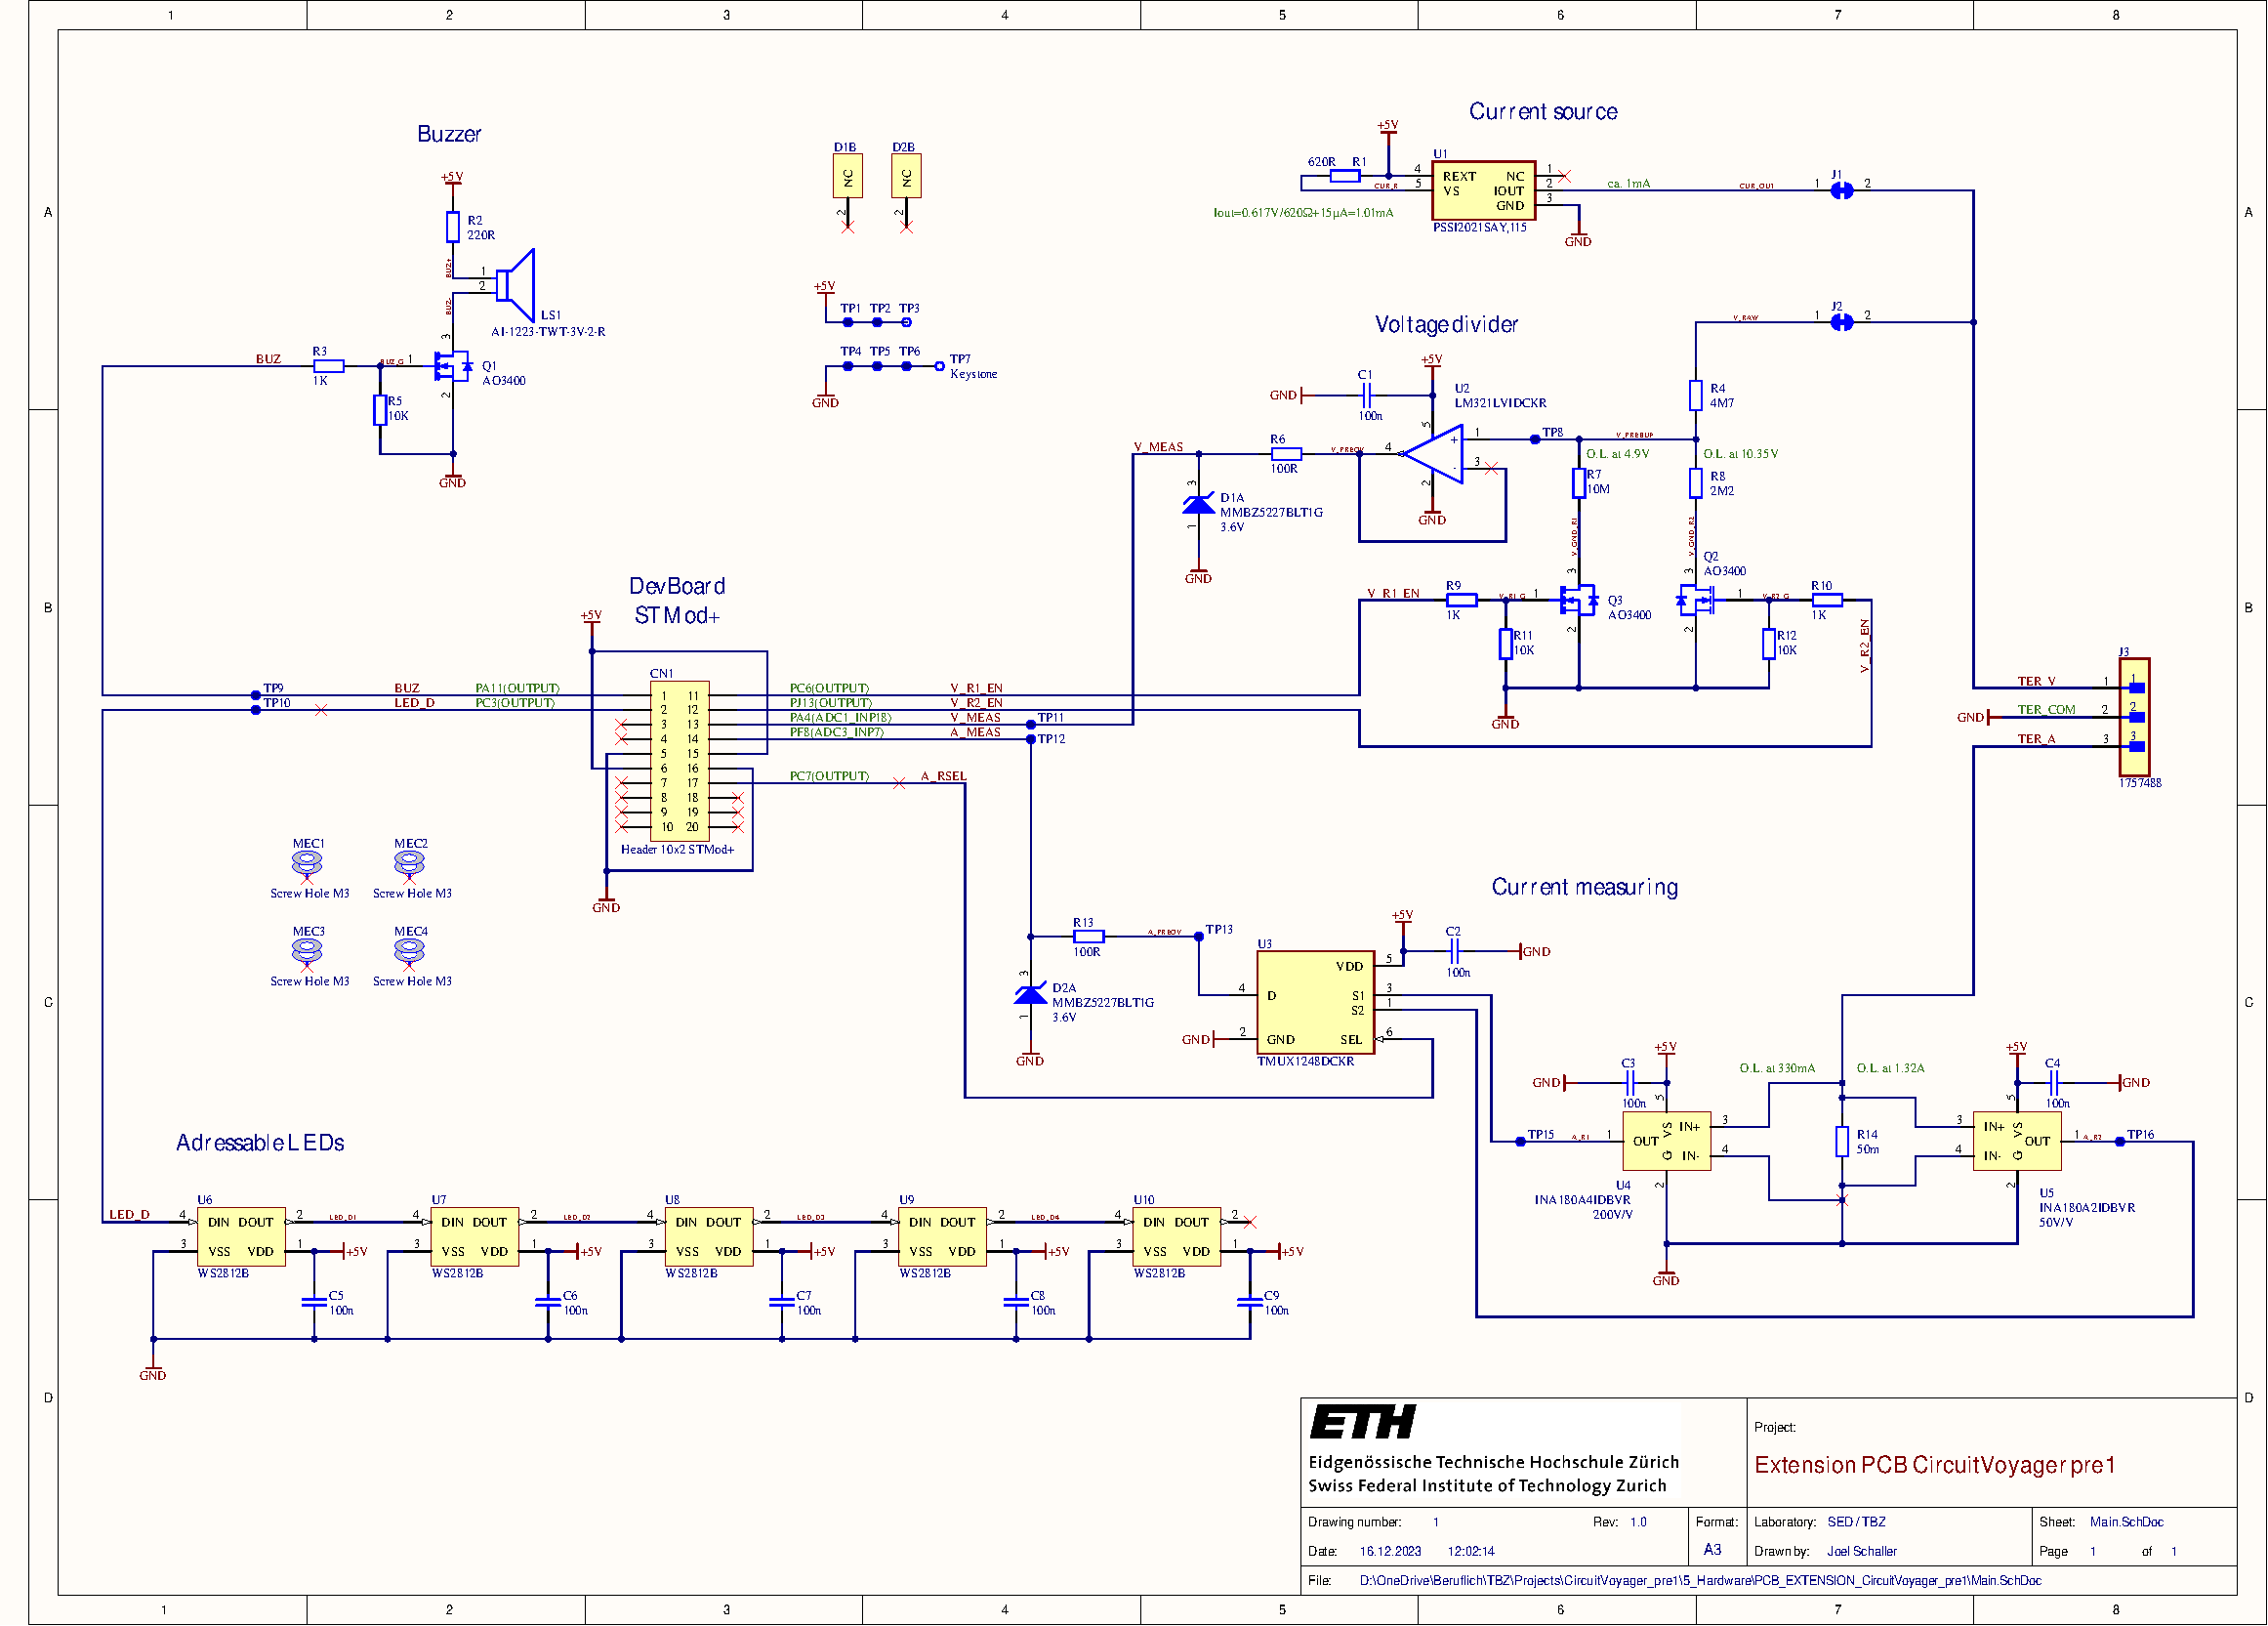
\includegraphics[width=6cm, trim={17cm 9.5cm 19cm 15.5cm}, clip]{../../../5_Hardware/PCB_EXTENSION_CircuitVoyager_pre1/Project Outputs for PCB_EXT_CV_PRE1/Schematic_PCB_EXTENSION_CircuitVoyager_pre1.pdf}
	\caption{Overvoltage Protection Circuit}
	\label{fig:Overvoltage Protection Circuit}
\end{figure}

My Problem is, that the voltages coming from  the Extension PCB, can't exceed 4V according to the MCUs datasheet. But because this PCB is powered by the 5V rail, theoretically these voltages could damage the MCU. So the goal was to develop a circuit which protects the ADC inputs. The first idea that came to my mind was to use varistors. I've already used the once in a project, but after reading some application notes on this topic, I decided to use a zenerdiode for the OVP. \cite{Protecting_ADC_Inputs_AN}

The zenerdiode I've used has a nominal zenervoltage of 3.6V (max. 3.78V) at 20mA. Together with R13 this should result with a maximum voltage of 3.78V at the ADC inputs. As long as the PREOV voltage doesn't exceed 5.6V.
\[U_{PREOV(MAX.)} = R_{13} \cdot I_Z + U_Z = 100\Omega \cdot 20mA + 3.6V = 5.6V\]
\[P_{R13} = R \cdot I^2 = 100\Omega \cdot (20mA)^2 = 40mW\]


\subsubsection{Voltage Divider Circuit}

\begin{figure}[H]
	\centering
	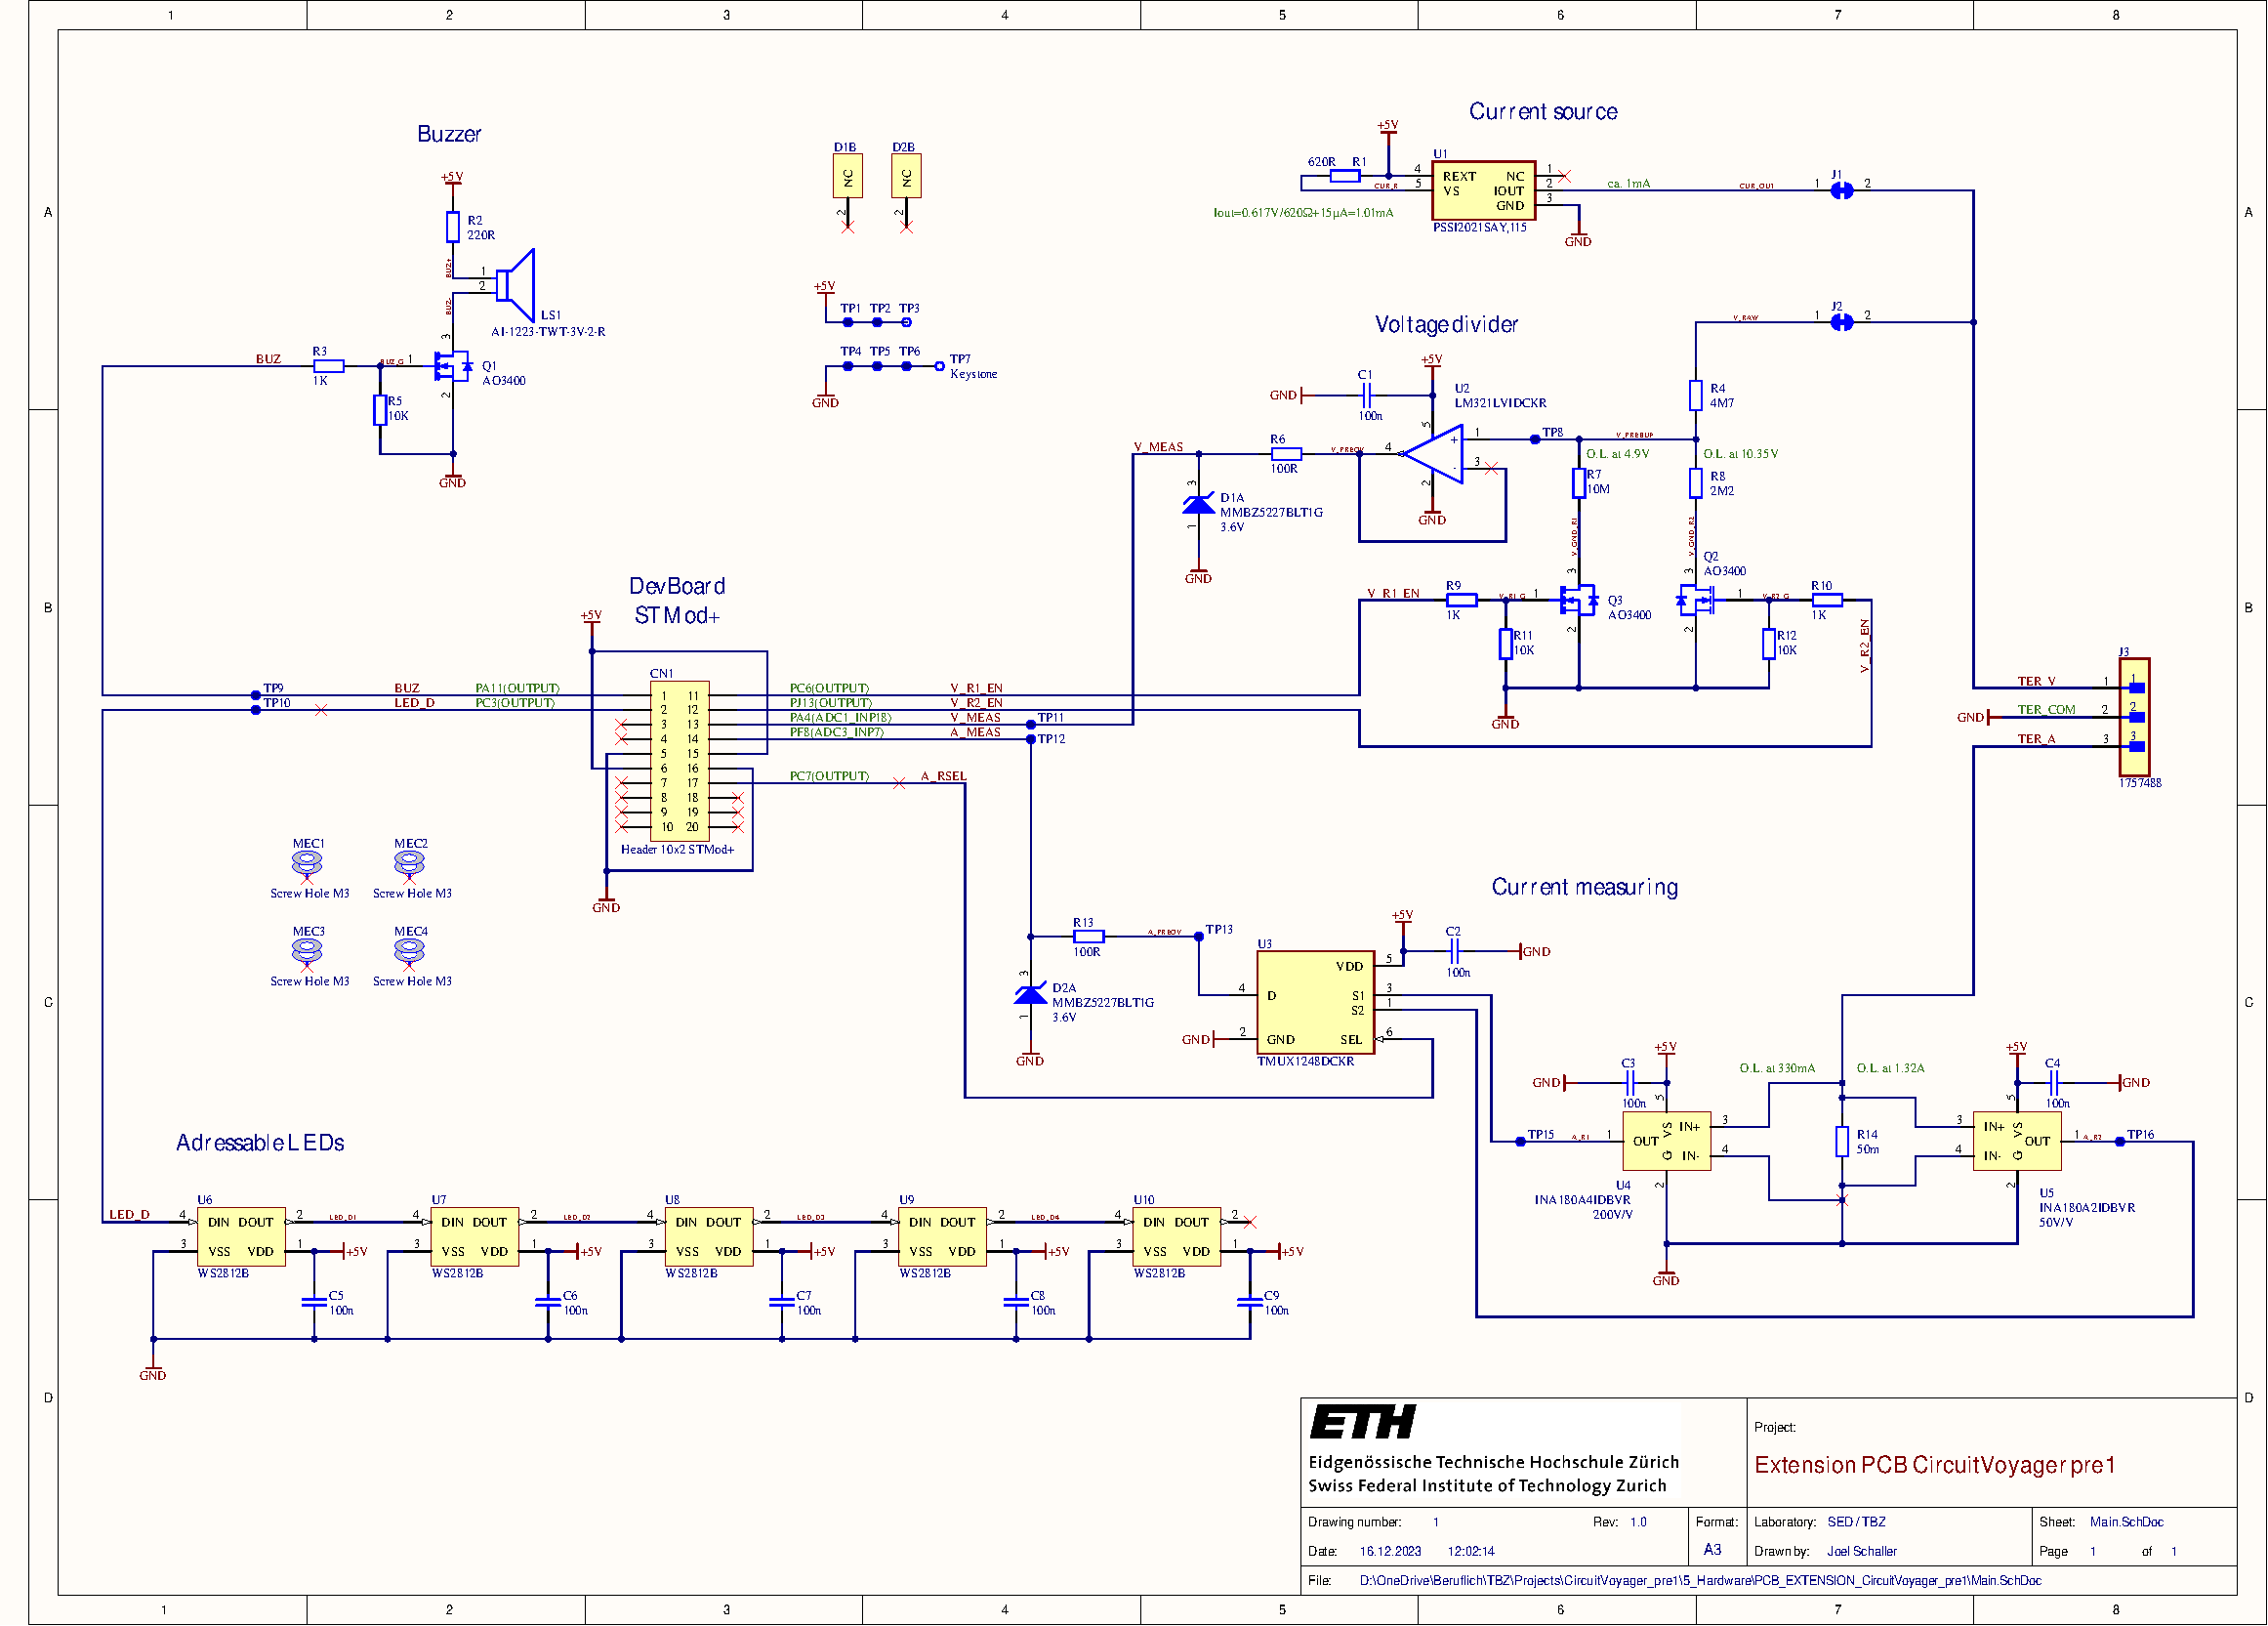
\includegraphics[width=12cm, trim={23cm 15cm 6cm 5cm}, clip]{../../../5_Hardware/PCB_EXTENSION_CircuitVoyager_pre1/Project Outputs for PCB_EXT_CV_PRE1/Schematic_PCB_EXTENSION_CircuitVoyager_pre1.pdf}
	\caption{Voltage Divider Circuit}
	\label{fig:Voltage Divider Circuit}
\end{figure}

The voltage divider is used to measure voltages over the V terminal. This circuit is one approach to range switching, which is described more detailed in the following chapter [Write more detailed text about how to execute range switching and what are the pros and cons. Minimum 3 options]. This voltage divider features 2 ranges and I came up with this idea by myself. The ranges are calculated as following:
\[U_{OL(R1)} = \frac{(R_4 + R_7) \cdot U_{OL(MCU)}}{R_7} = \frac{(4.7M\Omega + 10M\Omega) \cdot 3.3V}{10M\Omega} = 4.851V\]
\[U_{OL(R2)} = \frac{(R_4 + R_8) \cdot U_{OL(MCU)}}{R_8} = \frac{(4.7M\Omega + 2.2M\Omega) \cdot 3.3V}{2.2M\Omega} = 10.35V\]
This divided voltage is then fed into an impedance converter which guarantees that the voltage divider isn't manipulated by the ADC internal resistance and also helps on the DevBoards analog paths, because they're very long and therefore vulnerable to electromagnetic fields.

\textbf{
\begin{textbf}
Text to put into ranges part:
This range switching part has the advantage of using many ranges at once, as for example with 2 range switches can use 3 different ranges and with 3 range switches can use 7 ranges. On the other hand it has the disadvantage of only being able to divide the input voltage and not being able to amplify. Additionally, the internal resistance is always changing and therefore impacting the DUT. I wouldn't recommend this circuit because of said factors and only switch on the measured side. For example use different Amps / Divs to create the right voltage ranges and only switch the high Z path, that doesn't have an impact on the DUT.
\end{textbf}}




\subsubsection{Current Source Circuit}

\begin{figure}[H]
	\centering
	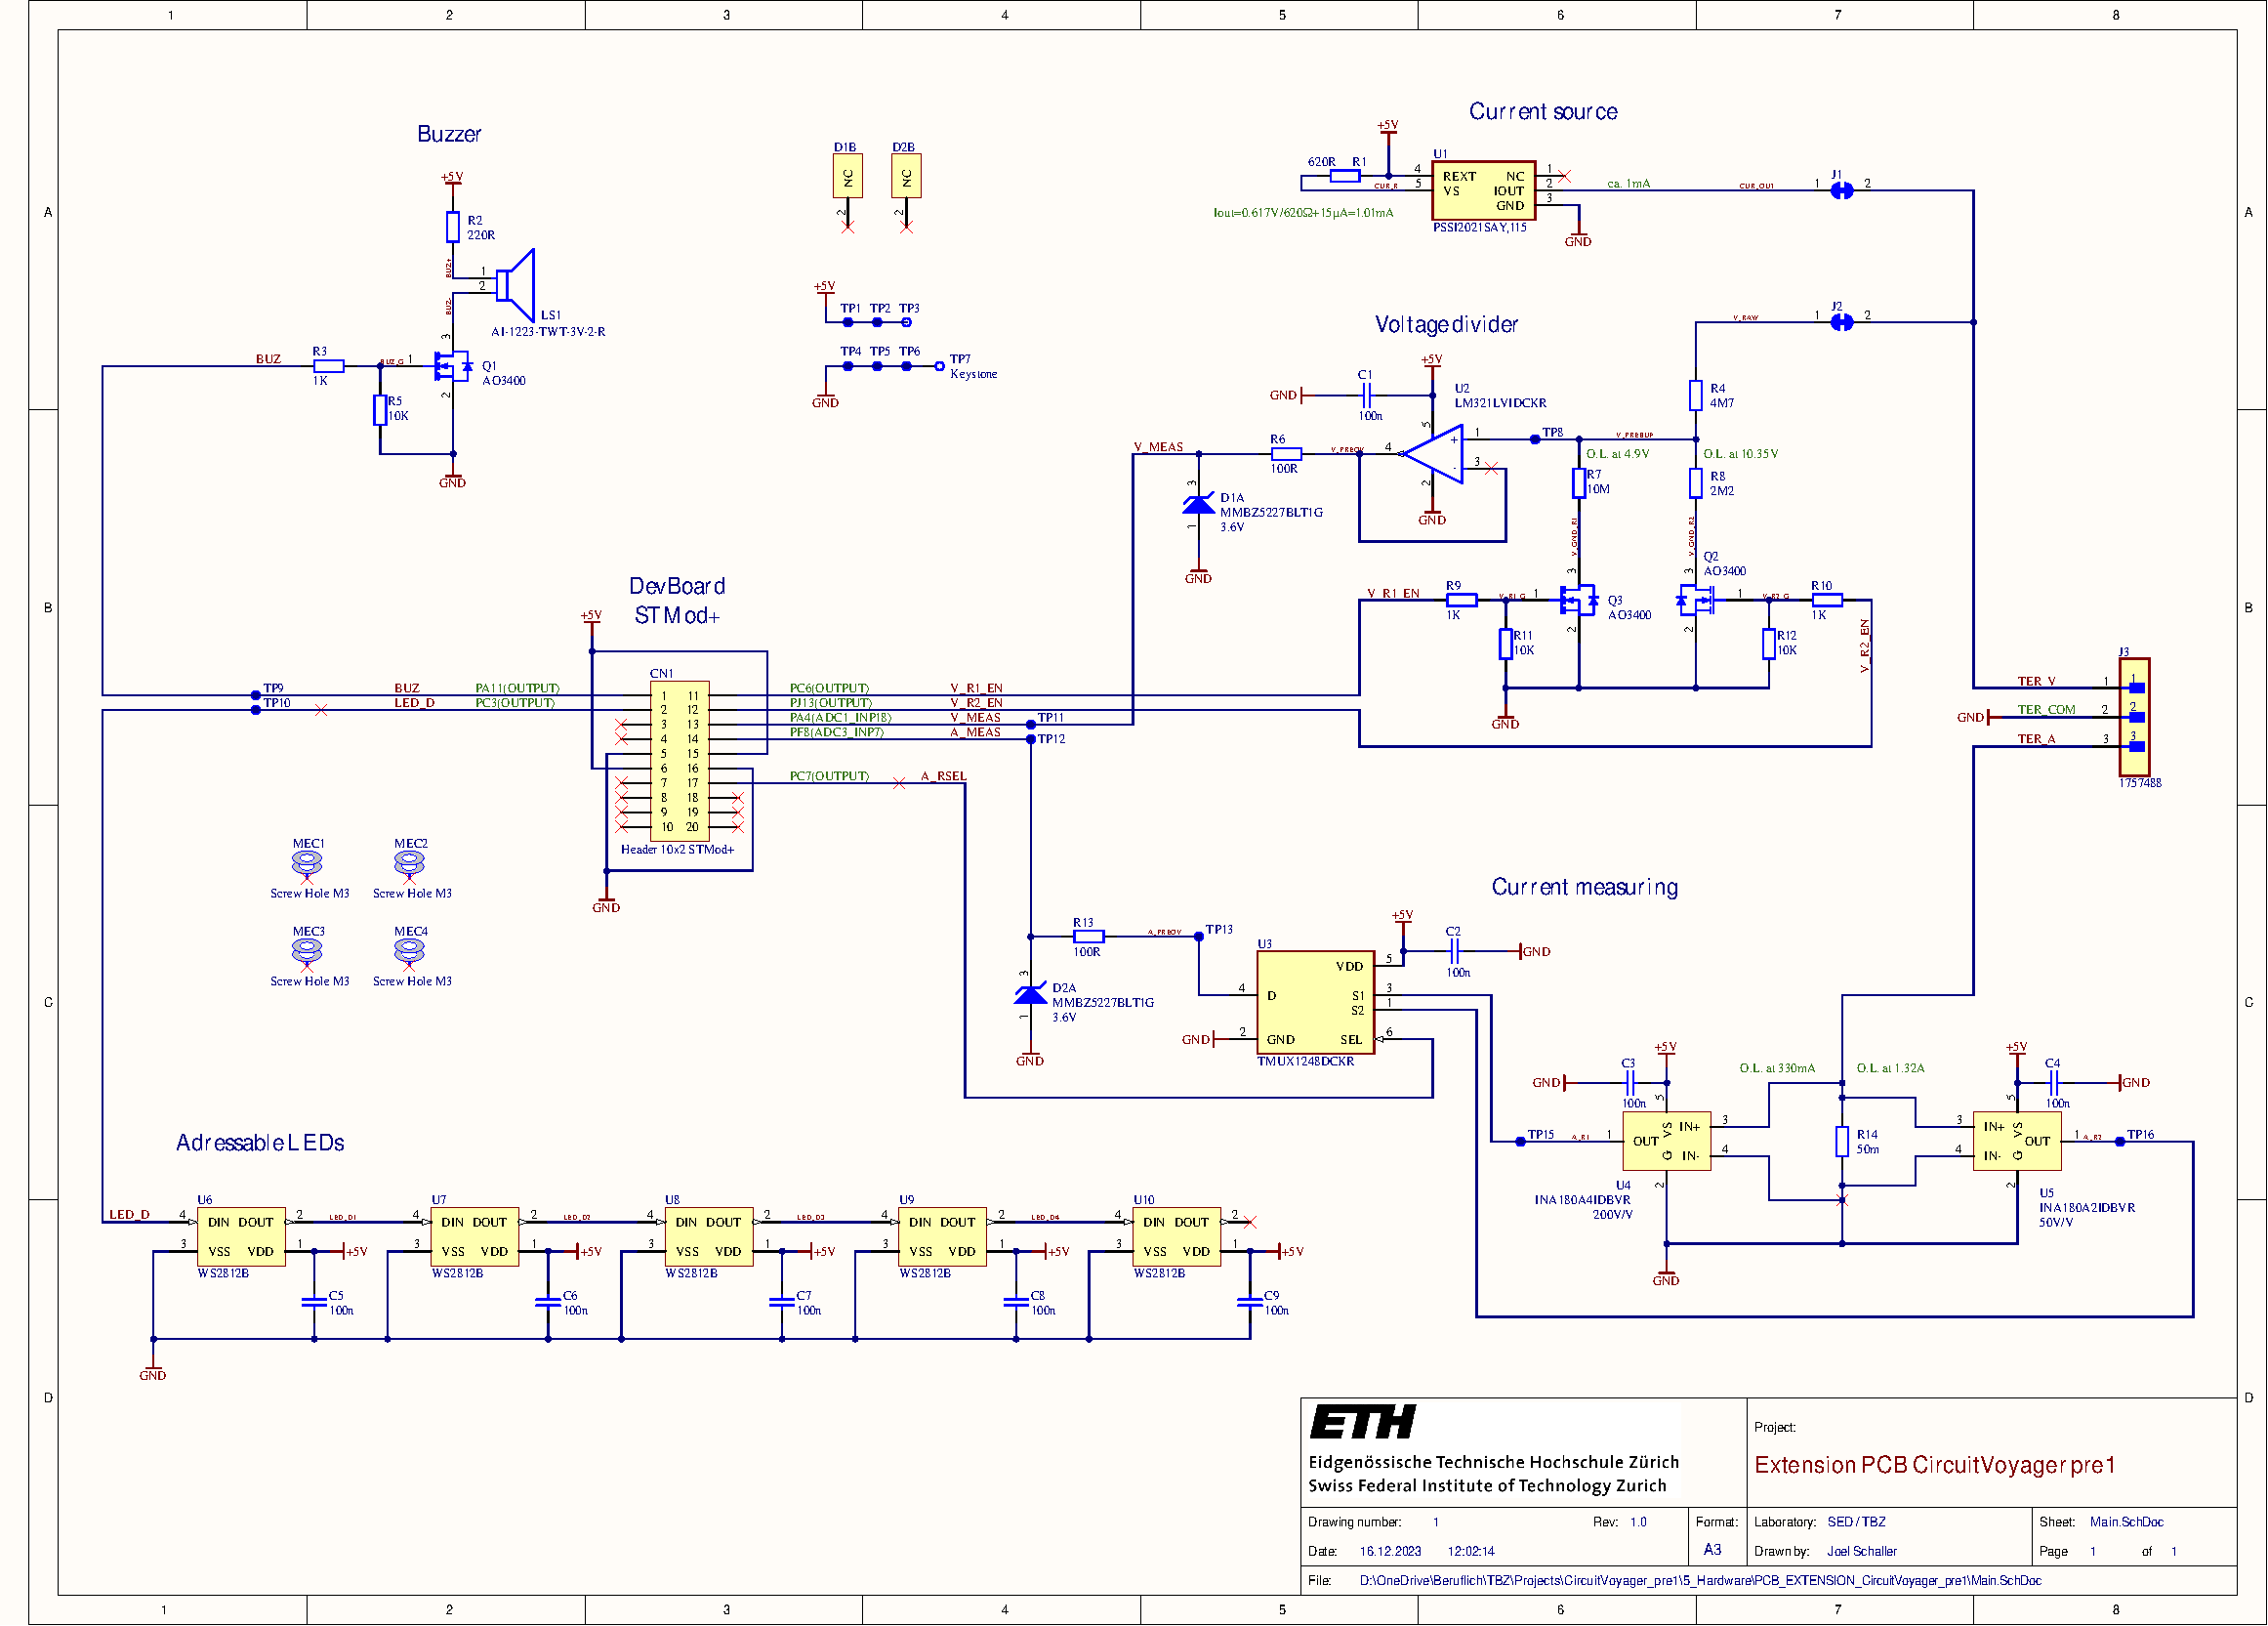
\includegraphics[width=10cm, trim={20cm 23cm 10cm 1cm}, clip]{../../../5_Hardware/PCB_EXTENSION_CircuitVoyager_pre1/Project Outputs for PCB_EXT_CV_PRE1/Schematic_PCB_EXTENSION_CircuitVoyager_pre1.pdf}
	\caption{Current Source Circuit}
	\label{fig:Current Source Circuit}
\end{figure}

The current source circuit will be used to measure continuity and resistance together with the voltage measuring function. A constant current will be induced to the DUT and because the voltage over the DUT can be measured, the resistance can be calculated. The constant current can be calculated as following:
\[I_{OUT} = \frac{U_{VS}}{R_1} + 15\mu A = \frac{0.617V}{620\Omega} + 15\mu A = 1.01mA\]
But this doesn't matter that much, because the DMM will be calibrated using the solderbridge J1.


\subsubsection{Current Measuring Circuit}

\begin{figure}[H]
	\centering
	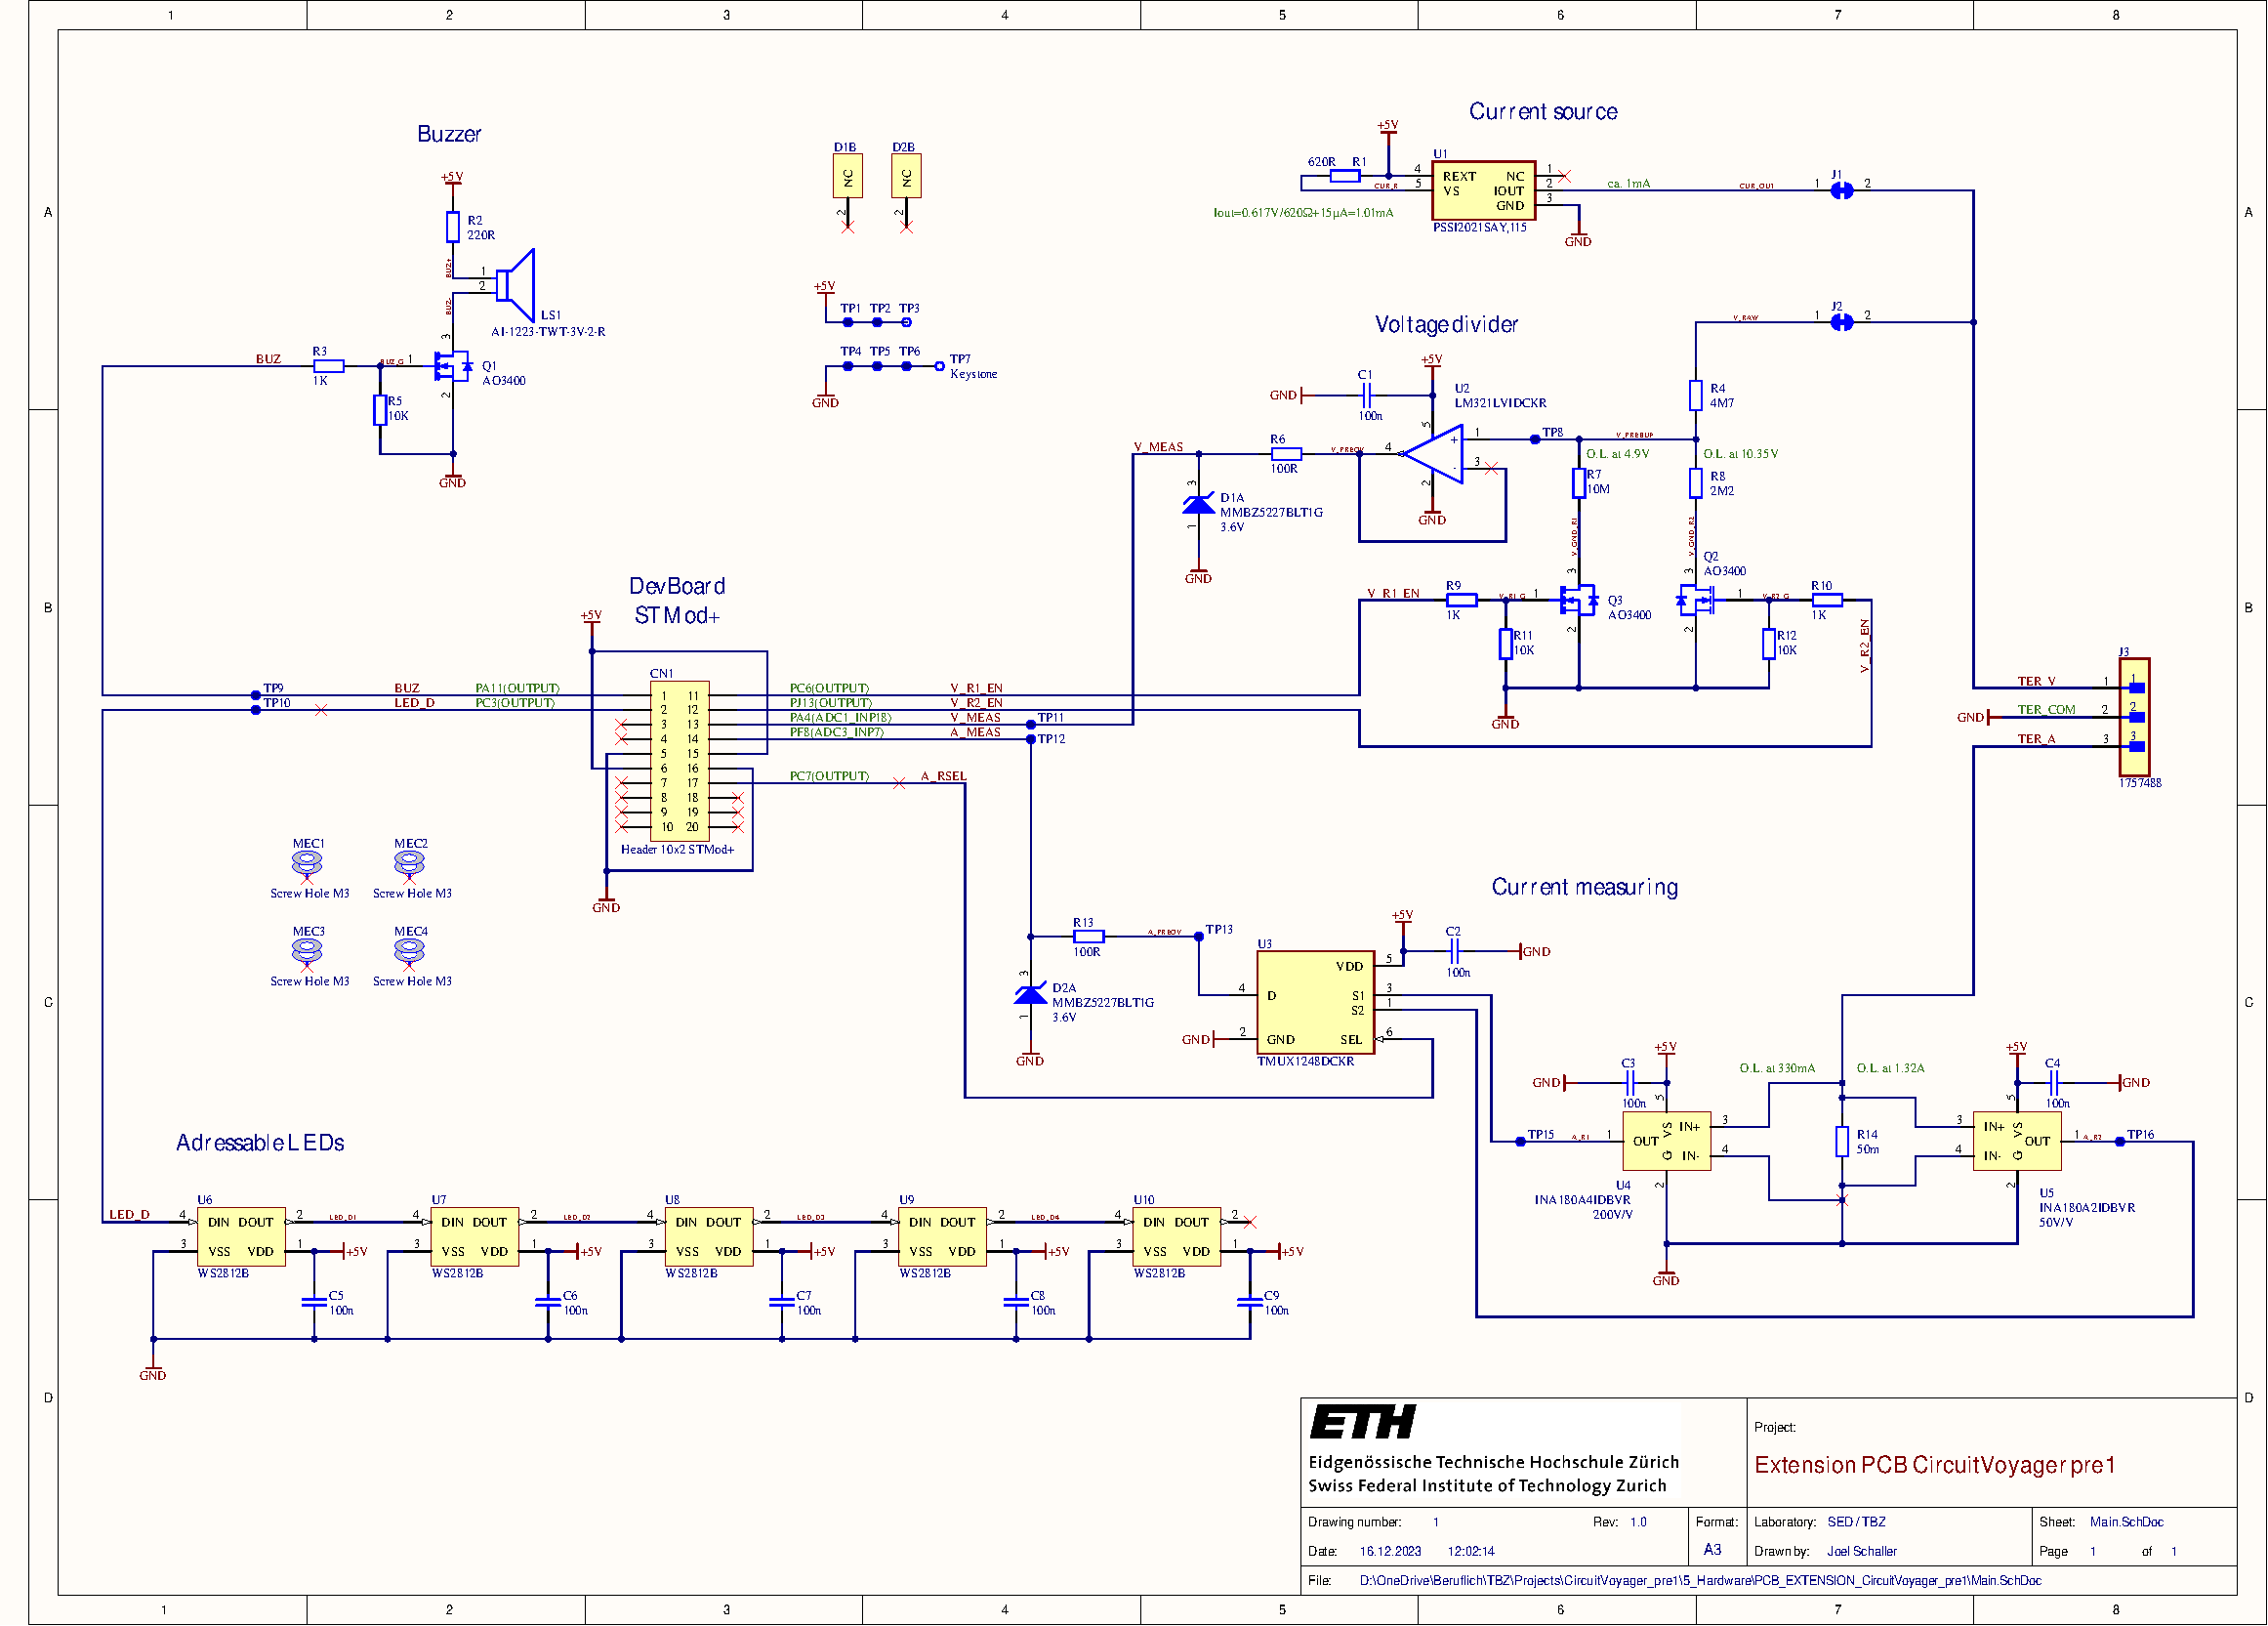
\includegraphics[width=14cm, trim={19.5cm 5cm 1cm 14.5cm}, clip]{../../../5_Hardware/PCB_EXTENSION_CircuitVoyager_pre1/Project Outputs for PCB_EXT_CV_PRE1/Schematic_PCB_EXTENSION_CircuitVoyager_pre1.pdf}
	\caption{Current Measuring Circuit}
	\label{fig:Current Measuring Circuit}
\end{figure}

The current measuring circuit is used to measure currents with the A terminal. This circuit is one approach to range switching, which is described more detailed in the following chapter [Write more detailed text about how to execute range switching and what are the pros and cons. Minimum 3 options]. This circuit features 2 ranges and I came up with this idea, while reading some articles on DMMs \cite{Digital_multimeter_circuit_using_ICL7107} \cite{AN-202_A_Digital_Multimeter_Using_the_ADD3501}. The ranges are calculated as following:
\[I_{OL(R1)} = \frac{U_{OL(MCU)}}{R_{14} \cdot G_{U4}} = \frac{3.3V}{50m\Omega \cdot 200\frac{V}{V}} = 330mA\]
\[I_{OL(R2)} = \frac{U_{OL(MCU)}}{R_{14} \cdot G_{U5}} = \frac{3.3V}{50m\Omega \cdot 50\frac{V}{V}} = 1.32A\]
These voltages are then fed into an analog MUX, which switches the processed voltages to the ADC. This has the advantage, that the DMM doesn't manipulate the actual path, where the current is flowing through and therefore not influencing the DUT.